

\subsection{Assignment of Trials to Conditions}
Here, we summarise the assignment of trials to conditions in Experiments 1 and 2, as described in the main paper:

\begin{center}
\begin{tabular}{l|llll}
\# of trials	& Experiment 1 & Experiment 2 \\ \hline
	2 & \textsc{One}  & \textsc{One}\\ \hline
	2 & \textsc{Two+Incompatible} & \textsc{Two+Incompatible}\\
	2 & \textsc{Two+Incompatible} & \textsc{Two+Compatible}\\ \hline
	2 & \textsc{Three+Incompatible} & \textsc{Three+Incompatible}\\
	2 & \textsc{Three+Incompatible} & \textsc{Three+Compatible}\\ \hline
	30 & Fillers & Fillers \\ \hline
\end{tabular}
\end{center}


\subsection{Coding of Conditions}

In the mixed-effects analyses, we used Contrast Coding to code conditions using three predictors:
One for the contrast between the \textsc{One} condition and the \textsc{Two}/\textsc{Three} conditions (\textsc{Embedding}),
one for the contrast between the \textsc{Two} and the \textsc{Three} condition (\textsc{Depth}),
and one for the contrast between \textsc{Compatible} and \textsc{Incompatible} (\textsc{Compatible}).
All predictors were centered.
This leads to the following coding:
\begin{center}
\begin{tabular}{l|llll}
	Condition	             & \textsc{Embedding} & \textsc{Depth} & \textsc{Compatible} \\ \hline
	\textsc{One} & -0.9   & 0  & 0 \\
	\textsc{Two}+\textsc{Incompatible} &  +0.1  & -0.5 & -0.5\\
		\textsc{Two}+\textsc{Compatible}             &  +0.1     &  -0.5    & +0.5\\
	\textsc{Three}+\textsc{Incompatible} & +0.1   & +0.5 & -0.5\\
		\textsc{Three}+\textsc{Compatible}             &   +0.1    &  +0.5    & +0.5\\
\end{tabular}
\end{center}
In Experiment 2, the fixed effects structure contained these fixed effects, Embedding Bias, and all non-degenerate\footnote{I.e., the interactions \textsc{Embedding}:\textsc{Depth} and \textsc{Embedding}:\textsc{Compatible} are not meaningful and omitted.} binary interactions.
In Experiment 1, main effects and interactions including compatibility were omitted.

Further, there were random effects for item, subjects, and nouns.
The random effects structure was the maximal structure justified by the experimental design~\citep{Barr2013RandomES}:
Items and participants had random slopes for all fixed effects.
Nouns had random slopes for all fixed effects not involving Embedding Bias (Embedding Bias is constant within each noun, so that per-noun slopes are not justified for it).


\subsection{Details for Data Analysis and Mixed-Effects Regression}\label{sec:regression-details}

We implemented models in Stan~\citep{carpenter2017stan} using \texttt{brms}~\citep{buerkner2017brms}.
Embedding Bias was centered.
Following \citet{buerkner2017brms}, the following prior was chosen.
Fixed effect coefficients had flat priors.
The intercept had a Student's $t$ prior with 3 degrees of freedom, scale $2.5$ and location $7$, where the location parameter was chosen based on the mean log reading time in preceding studies (Section~\ref{sec:previous}).
Covariance matrices for random effects were parameterized as the combination of a correlation matrix and a vector of standard deviations \citep{barnard2000modeling}.
Correlation matrices had $LKJ(1)$ priors~\citep{lewandowski2009generating}.
The standard deviations for random effects and for the residuals had Student's $t$ priors with 3 degrees of freedom, scale $2.5$, and location $0$.
See the meta-analysis in Section~\ref{sec:meta} with Figure~\ref{fig:meta-regularizing} for an analysis with a more strongly regularizing prior.

Posterior inference used the NUTS sampler \citep{homan2014the} implemented in Stan.
We ran four chains with 8000 iterations each, of which the first half were discarded as warmup samples.
Convergence was assessed using $\widehat{R}$ and visual inspection of chains.

\subsection{Effects in Raw Reading Times}\label{sec:effects-raw-rt}
Here, we detail how we derived posteriors for effects in raw reading times from the Bayesian mixed-effects model.

We compute the effect of Depth in raw reading times:
\begin{enumerate}
	\item Reading time in the \textsc{Two} condition: $R_{\textsc{Two}} = \exp(\alpha + 0.1 \cdot \beta_{\textsc{Embedding}} - 0.5 \cdot \beta_{\textsc{Depth}})$
	\item Reading time in the \textsc{Three} condition: $R_{\textsc{Three}} = \exp(\alpha + 0.1 \cdot \beta_{\textsc{Embedding}} + 0.5 \cdot \beta_{\textsc{Depth}})$
\end{enumerate}
Then the effect of Depth is given as:
\begin{equation}
	\widehat{\Delta}_{Depth} = R_{\textsc{Three}} - R_{\textsc{Two}}
\end{equation}
Next, the effect of compatibility is given as
\begin{equation}
	\widehat{\Delta}_{\textsc{Compatibility}} = R_{\textsc{Compatible}} - R_{\textsc{Incompatible}}
\end{equation}
where
\begin{enumerate}
	\item Reading time in the \textsc{Compatible} conditions: $R_{\textsc{Compatible}} = \exp(\alpha + 0.1 \cdot \beta_{\textsc{Embedding}} + 0.5 \cdot \beta_{\textsc{Compatible}})$
	\item Reading time in the \textsc{Incompatible} conditions: $R_{\textsc{Incompatible}} = \exp(\alpha + 0.1 \cdot \beta_{\textsc{Embedding}} - 0.5 \cdot \beta_{\textsc{Compatible}})$
\end{enumerate}

For Figure 3 in the main paper, the reading time for ``\emph{fact}'' (similarly ``\emph{report}'') in \textsc{One}  (similarly for the other conditions) is given as\footnote{Similar results are obtained when also taking into account the random effects for fact/report.}
\begin{equation}
	\exp(\alpha - 0.1 \beta_{\textsc{Embedding}} + \beta_{\textsc{EmbeddingBias}} E_{fact} - 0.1 \beta_{\textsc{Embedding}:\textsc{EmbeddingBias}} E_{fact})
\end{equation}
where $E_{fact}$ denotes the centered embedding bias of ``fact''.
We obtained posteriors for these effect sizes by transforming the posterior samples for the coefficients.
Figure 3 in the main paper shows the mean and standard deviation of these posteriors.

\subsection{Results for Experiments 1 and 2}
\paragraph{Details on Participant Recruitment}
Participants were recruited on Prolific (\url{prolific.co}). The task, advertised as ``Read English Sentences by Pressing Keys'', was only shown to residents of the US or the UK with English listed as their first language.
Participants were asked what they considered adequate pay for the task, and listed amounts generally consistent with the pay offered.
Data was collected by submitting a packet of data to a server upon completion of every sentence.
For a small number of participants, less than 10 critical trials arrived at the server, either because they dropped out of the experiment or because not all packets of data were submitted successfully to the server.
Those participants were paid, and their data were not excluded.
In Experiment 1, data from one participant was not submitted to the server and lost entirely.
In Experiment 2, experimenter error led to 17 extra participants being recruited. Their data is excluded when analyzing results specifically for Experiment 2 for consistency, but included in the pooled meta-analysis (Section~\ref{sec:meta} and Figure~\ref{fig:meta}).
This exclusion decision does not affect the qualitative or quantitative conclusions of the mixed-effects analysis.

\paragraph{Mixed-Effects Models}
We report the mixed-effects models for Experiments 1 and 2 in Figures~\ref{fig:expt1-fixed-effects}-\ref{fig:expt2-fixed-effects}.

We note that the data from Experiments 1--2 do not provide conclusive evidence for an effect of Embedding Bias or Compatibility within specifically the \textsc{Two} condition. 
Substantial evidence for such effects within \textsc{Two} is, however, provided when pooling data across these and previous studies, see Section~\ref{sec:meta} and Figure~\ref{fig:meta}.




\begin{figure}
    \centering
    

	\textbf{Fixed Effects Estimates}
	\begin{tabular}{cc}
	Main Effects & Interactions \\
		\includegraphics[width=0.48\textwidth]{../resource-rational-surprisal/experiments/maze/experiment1/Submiterator-master/figures/posterior-histograms-main_effects.pdf} &
	\includegraphics[width=0.48\textwidth]{../resource-rational-surprisal/experiments/maze/experiment1/Submiterator-master/figures/posterior-histograms-interactions.pdf}
 	\end{tabular}
  
	\textbf{Effects in Raw Reading Times}

 \includegraphics[width=0.48\textwidth]{../resource-rational-surprisal/experiments/maze/experiment1/Submiterator-master/figures/posterior-histograms-RawEffects.pdf}
  
   
	\caption{Top: Mixed-effects analysis of log-transformed reading times on the critical word in Experiment 1. We plot the posterior densities for the fixed effects coefficients, with symmetric 95\% credible intervals. The key effects of theoretical interest are Depth and the interaction Embedding:EmbeddingBias. Bottom: Effects in raw reading times. Compare Figure~\ref{fig:meta} for a meta-analysis pooling all available evidence.}
    \label{fig:expt1-fixed-effects}
\end{figure}






\begin{figure}
    \centering
    

	\textbf{Fixed Effects Estimates}
	\begin{tabular}{cc}
	Main Effects & Interactions \\
		\includegraphics[width=0.48\textwidth]{../resource-rational-surprisal/experiments/maze/experiment2/Submiterator-master/figures/posterior-histograms-main_effects.pdf} &
	\includegraphics[width=0.48\textwidth]{../resource-rational-surprisal/experiments/maze/experiment2/Submiterator-master/figures/posterior-histograms-interactions.pdf}
	\end{tabular}
  
	\textbf{Effects in Raw Reading Times}

	\includegraphics[width=0.48\textwidth]{../resource-rational-surprisal/experiments/maze/experiment2/Submiterator-master/figures/posterior-histograms-RawEffects.pdf}


	\caption{Top: Mixed-effects analysis of log-transformed reading times on the critical word in Experiment 2. We plot the posterior densities for the fixed effects coefficients, with symmetric 95\% credible intervals. The key effects of theoretical interest are Depth, Compatible, and the interaction Embedding:EmbeddingBias. Bottom: Posteriors for effects in raw reading times. Compare Figure~\ref{fig:meta} for a meta-analysis pooling all available evidence.}
    \label{fig:expt2-fixed-effects}
\end{figure}





\subsection{Analysis of Incorrect Responses}
Figure~\ref{fig:expt2-errors} shows error rates by word number and participants in the pooled data from Section~\ref{sec:meta}.
Error rates are similar to~\citet{boyce2020maze}, and most participants make errors on less than 5\% of words.



\begin{figure}
    \centering
    
    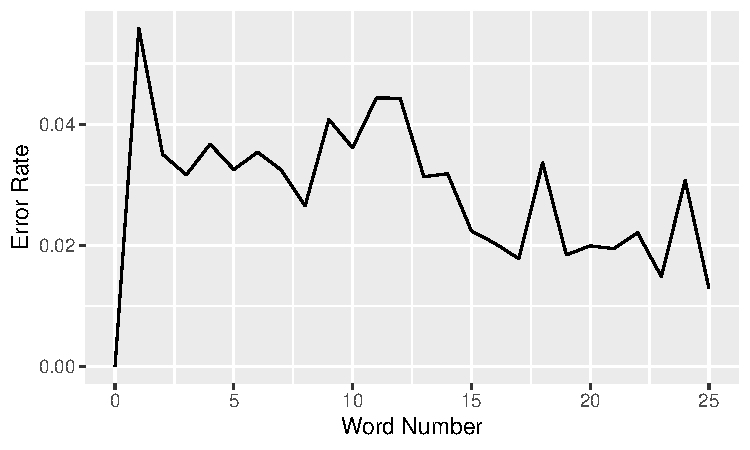
\includegraphics[width=0.48\textwidth]{../resource-rational-surprisal/experiments/maze/meta/figures/errors-by-position.pdf}
   % 
     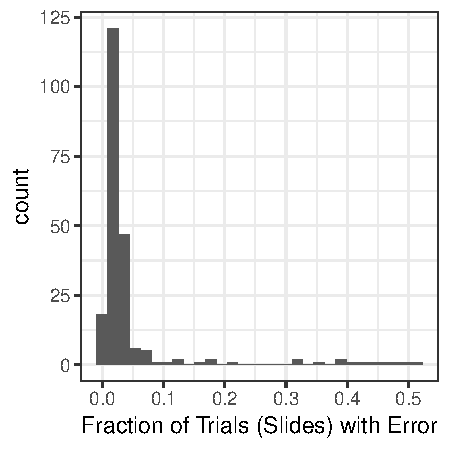
\includegraphics[width=0.38\textwidth]{../resource-rational-surprisal/experiments/maze/meta/figures/slides-errors.pdf}
   
	\caption{Error rates in the pooled data from Section~\ref{sec:meta}. Left: Error rates by position in the sentence (before applying exclusion criteria). For comparison, \citet{boyce2020maze} report an error rate of 10\% on the second word, and about 2--3\% for words at position $\geq 5$. Right: Fraction of words with error by participant. The vast majority of participants makes errors on less than 5\% of words. The exclusion criterion affects participants making errors on more than 20\% of words.}
    \label{fig:expt2-errors}
\end{figure}



\paragraph{Errors across Conditions}
We analyzed answer correctness on the critical verb using the same fixed and random effects as we used for reading times, but with a logistic model, again implemented in \texttt{brms} with default priors.
We conducted analyses on the pooled data as in Section~\ref{sec:meta}.
Results are shown in Figure~\ref{fig:expt2-errors-brms}.
Errors increase in the difficult \textsc{Three} condition, as shown by the effect of \textsc{Depth}. No other patterns find significant statistical support.

\begin{figure}
    \centering
    
	\textbf{Fixed Effects Estimates}
	\begin{tabular}{cc}
	Main Effects & Interactions \\
		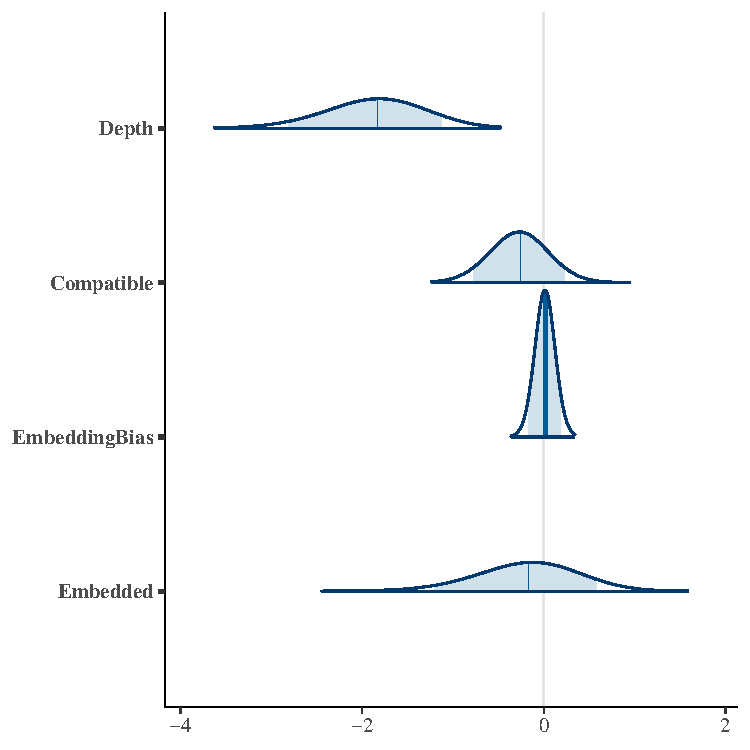
\includegraphics[width=0.48\textwidth]{../resource-rational-surprisal/experiments/maze/meta/figures/analyze_Errors_R_posterior-histograms-main_effects.pdf} &
     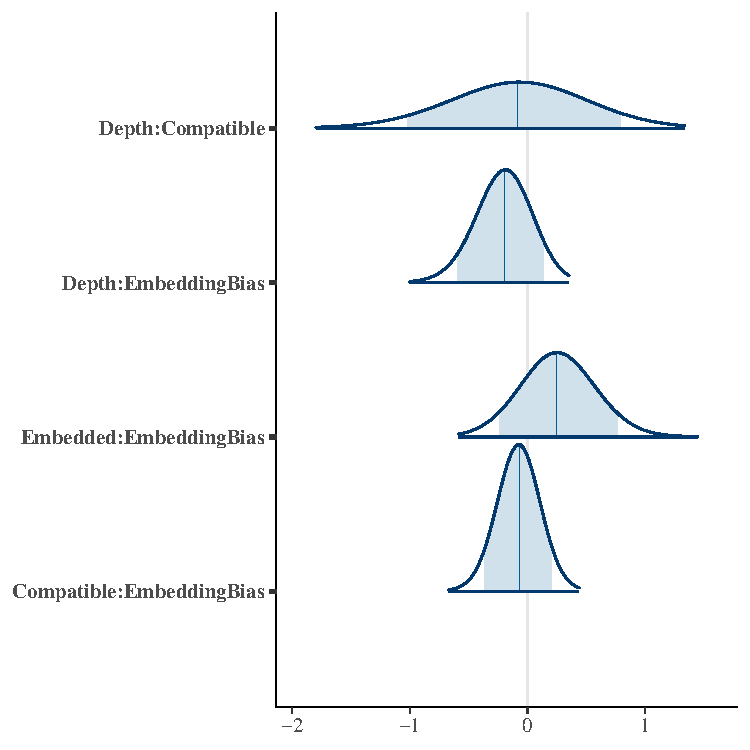
\includegraphics[width=0.48\textwidth]{../resource-rational-surprisal/experiments/maze/meta/figures/analyze_Errors_R_posterior-histograms-interactions.pdf}
	\end{tabular}
   
	\caption{Logistic mixed-effects analysis of errors on the critical word in the pooled data from Section~\ref{sec:meta}. Errors increase in the difficult \textsc{Three} condition. No other patterns find statistical support.}
    \label{fig:expt2-errors-brms}
\end{figure}




\paragraph{Reading Times conditioned on Errors}
We also conducted a version of the analysis on trials with both correct and incorrect responses, where we added a fixed effect for response correctness, and interactions with the predictors of primary theoretical interest, i.e., Compatible and Embedding Bias.
Again, we report analyses on the pooled data as in Section~\ref{sec:meta}.
The resulting model fit is shown in Figure~\ref{fig:expt2-with-errors-brms}.
There was a main effect of response correctness such that correct responses tend to be faster than incorrect ones, suggesting that errors reflect processing difficulty. 
Effects of Embedding Bias and Compatibility continue to be estimated very similarly to the model fitted on only correct trials (Figure~\ref{fig:meta} in Section~\ref{sec:meta}).


\begin{figure}
    \centering
   
	\textbf{Fixed Effects Estimates}
	\begin{tabular}{cc}
	Main Effects & Interactions \\
		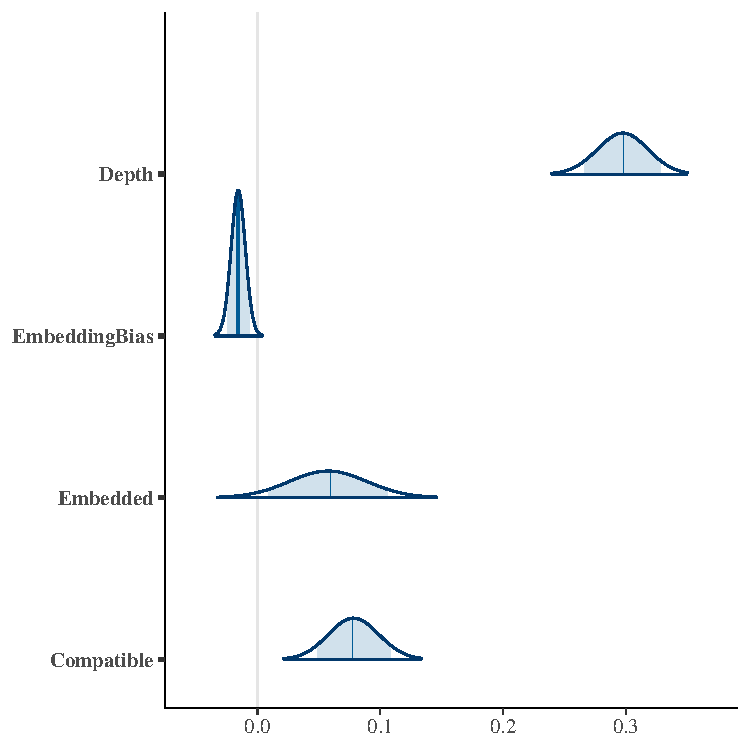
\includegraphics[width=0.48\textwidth]{../resource-rational-surprisal/experiments/maze/meta/figures/analyze_WithErrors_R_posterior-histograms-main_effects.pdf} &
     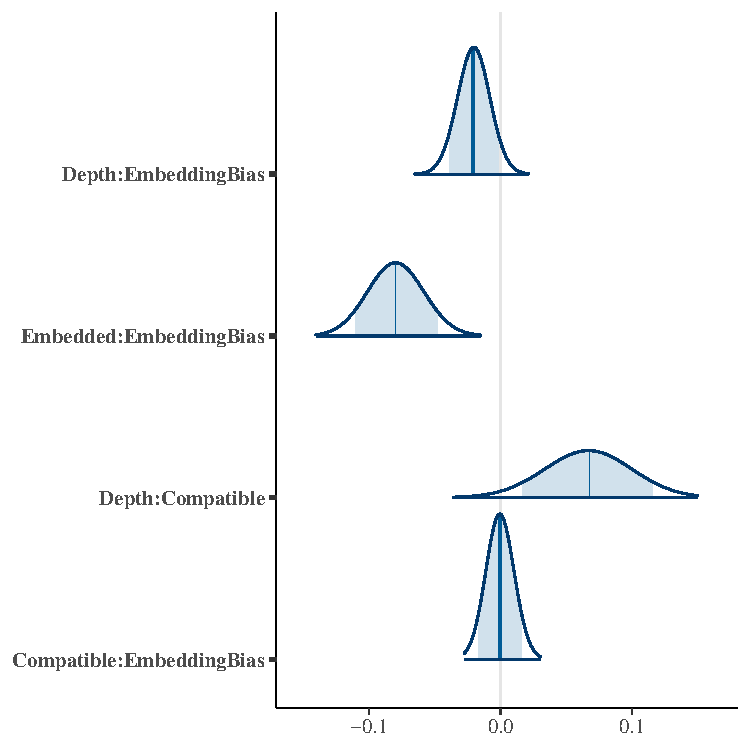
\includegraphics[width=0.48\textwidth]{../resource-rational-surprisal/experiments/maze/meta/figures/analyze_WithErrors_R_posterior-histograms-interactions.pdf}
	\end{tabular}

	Effects and Interactions involving Response Correctness

      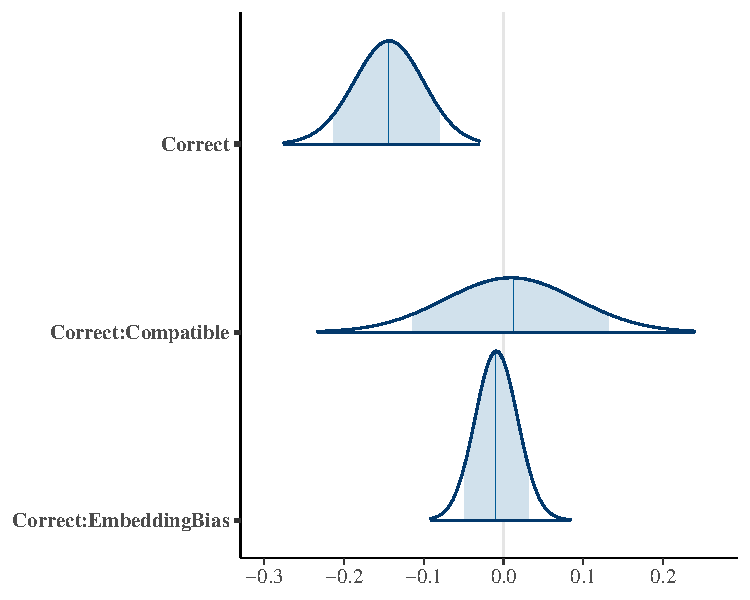
\includegraphics[width=0.48\textwidth]{../resource-rational-surprisal/experiments/maze/meta/figures/analyze_WithErrors_R_posterior-histograms-interactionsWithCorrect.pdf}
  
	\caption{Experiment 2: Mixed-effects analysis of reading times on the critical word in the data from Section~\ref{sec:meta}, including trials with an incorrect response, conditioned on response correctness. Correct responses tend to be faster than incorrect ones (main effect of \textsc{Correct}), suggesting that difficulty can manifest in both high reading times and incorrect responses. Response correctness did not impact the effects of compatibility or embedding bias. Compare Figure~\ref{fig:meta} in Section~\ref{sec:meta} for the corresponding analysis on the correct trials only.}
    \label{fig:expt2-with-errors-brms}
\end{figure}



\subsection{Effect of Outlier Removal}\label{sec:outliers}

Reaction time experiments can produce outliers, particularly due to repeated button pressing or due to participants being distracted or taking a break during a trial.
Across the pooled data in Section~\ref{sec:meta}, the minimum and maximum reading times recorded were 1 ms and 14 min, presumably due to rapid button presses and pauses within the experiment, respectively.
As described in the main paper, we addressed this by excluding the top and bottom 1\% of reading times (across critical items and fillers) from the dataset before every mixed-effects analysis.  The resulting thresholds for exclusions (first and 99th percentile) were 428 ms and 3.5 s, respectively.
2.5\% of the trials excluded due to this criterion were in the critical region, corresponding to 3.2\% of the trials in the critical region.

We alternatively considered a more permissive criterion, where we removed reading times below 200 ms (percentile: 0.3\%) and above 10 s (percentile: 99.9\%).
Results are similar to those from the other analysis, with larger effect sizes and sometimes stronger statistical evidence for our conclusions; we show those for Experiments 1 and 2 in Figures~\ref{fig:expt1-fixed-effects-outliers}--\ref{fig:expt2-fixed-effects-outliers}.








\begin{figure}
    \centering
    

	\textbf{Fixed Effects Estimates}
	\begin{tabular}{cc}
	Main Effects & Interactions \\
		\includegraphics[width=0.48\textwidth]{../resource-rational-surprisal/experiments/maze/experiment1/Submiterator-master/figures/posterior-histograms-main_effects_Outliers.pdf} &
	\includegraphics[width=0.48\textwidth]{../resource-rational-surprisal/experiments/maze/experiment1/Submiterator-master/figures/posterior-histograms-interactions_Outliers.pdf}
 	\end{tabular}
  
	\textbf{Effects in Raw Reading Times}

 \includegraphics[width=0.48\textwidth]{../resource-rational-surprisal/experiments/maze/experiment1/Submiterator-master/figures/posterior-histograms-RawEffects_Outliers.pdf}
  
   
	\caption{Alternative outlier removal: Mixed-effects analyses for Experiment 1, with more permissive outlier removal (removing reaction times below 200ms and above 10s, see Section~\ref{sec:outliers}). Compare Figure~\ref{fig:expt1-fixed-effects} for results with another criterion (removing top and bottom 1\%). Statistical evidence for the key effects (Depth and the interaction Embedding:EmbeddingBias) is similar to the analysis in Figure~\ref{fig:expt1-fixed-effects}, though effect size estimates are higher than in Figure~\ref{fig:expt1-fixed-effects}.}
    \label{fig:expt1-fixed-effects-outliers}
\end{figure}








\begin{figure}
    \centering
    

	\textbf{Fixed Effects Estimates}
	\begin{tabular}{cc}
	Main Effects & Interactions \\
		\includegraphics[width=0.48\textwidth]{../resource-rational-surprisal/experiments/maze/experiment2/Submiterator-master/figures/posterior-histograms-main_effects_Outliers.pdf} &
	\includegraphics[width=0.48\textwidth]{../resource-rational-surprisal/experiments/maze/experiment2/Submiterator-master/figures/posterior-histograms-interactions_Outliers.pdf}
 	\end{tabular}
  
	\textbf{Effects in Raw Reading Times}

 \includegraphics[width=0.48\textwidth]{../resource-rational-surprisal/experiments/maze/experiment2/Submiterator-master/figures/posterior-histograms-RawEffects_Outliers.pdf}
  
   
	\caption{Alternative outlier removal: Mixed-effects analyses for Experiment 2, with more permissive outlier removal (removing reaction times below 200ms and above 10s, see Section~\ref{sec:outliers}). Compare Figure~\ref{fig:expt2-fixed-effects} for results with another criterion (removing top and bottom 1\%). Statistical evidence for the key effects (Depth, Compatible, and the interaction Embedding:EmbeddingBias) is similar to the analysis in Figure~\ref{fig:expt2-fixed-effects}, though effect size estimates are higher than in Figure~\ref{fig:expt2-fixed-effects}.}
    \label{fig:expt2-fixed-effects-outliers}
\end{figure}


